% ============================================================================
% CHAPTER 4: ACTIVATION FUNCTIONS AND SIGMOID NEURONS
% ============================================================================

\chapter{Activation Functions and Sigmoid Neurons}
\label{ch:activation_functions}

% ============================================================================
% OVERVIEW
% ============================================================================

\section{Chapter Overview}

This chapter introduces the crucial concept of \textbf{activation functions}---the nonlinear transformations that give neural networks their power. We focus particularly on the sigmoid function, understand why smooth activation functions are preferable to step functions, and explore the forward pass through a neural network.

\textbf{Learning Objectives:}
\begin{itemize}
    \item Understand why activation functions are necessary
    \item Compare step functions with smooth alternatives
    \item Master the sigmoid function and its properties
    \item Implement the forward pass through a network
    \item Compute loss functions (Mean Squared Error)
\end{itemize}

% ============================================================================
% THE NEED FOR SMOOTH ACTIVATIONS
% ============================================================================

\section{From Step Functions to Smooth Activations}

\subsection{Problems with the Step Function}

Recall the perceptron's activation function:
\[
g(z) = \begin{cases} 1 & \text{if } z \geq 0 \\ 0 & \text{otherwise} \end{cases}
\]

This step function has significant drawbacks:

\begin{enumerate}
    \item \textbf{Not differentiable}: The step function has an undefined derivative at $z = 0$ and zero derivative everywhere else. This prevents gradient-based learning.
    
    \item \textbf{Non-smooth}: Small changes in weights can cause large jumps in output.
    
    \item \textbf{No gradient signal}: When $z \neq 0$, the derivative is zero, providing no information about how to improve weights.
\end{enumerate}

\begin{bluebox}[Why Differentiability Matters]
Modern neural network training relies on \textbf{gradient descent}---an optimization algorithm that uses derivatives to find optimal weights. If the activation function isn't differentiable, we cannot compute how changes in weights affect the output, making learning impossible.

The derivative tells us: ``If I increase this weight by a tiny amount, how much will the output change?'' This information is essential for learning.
\end{bluebox}

\subsection{Desirable Properties of Activation Functions}

An ideal activation function should be:

\begin{enumerate}
    \item \textbf{Smooth (continuous)}: No jumps or discontinuities
    \item \textbf{Differentiable}: Has a well-defined derivative everywhere (or almost everywhere)
    \item \textbf{Nonlinear}: Without nonlinearity, neural networks collapse to linear models
    \item \textbf{Bounded outputs}: Prevents exploding activations (for some functions)
    \item \textbf{Computationally efficient}: Fast to compute
\end{enumerate}

% ============================================================================
% THE SIGMOID FUNCTION
% ============================================================================

\section{The Sigmoid Function}

\subsection{Definition}

\begin{definitionbox}[Sigmoid Function]
The \textbf{sigmoid function} (also called the logistic function) is defined as:
\[
\sigma(z) = \frac{1}{1 + e^{-z}}
\]
where $z = \vect{w}^\top \vect{x} + b$ (the weighted sum plus bias).
\end{definitionbox}

\subsection{Properties of Sigmoid}

\begin{center}
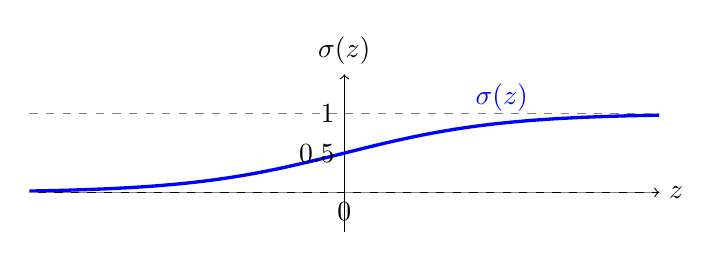
\begin{tikzpicture}
    \draw[->] (-4,0) -- (4,0) node[right] {$z$};
    \draw[->] (0,-0.5) -- (0,1.5) node[above] {$\sigma(z)$};
    
    % Sigmoid curve
    \draw[very thick, blue, domain=-4:4, samples=100] plot (\x, {1/(1+exp(-\x))});
    
    % Asymptotes
    \draw[dashed, gray] (-4,1) -- (4,1);
    \draw[dashed, gray] (-4,0) -- (4,0);
    
    % Labels
    \node[left] at (0,1) {$1$};
    \node[left] at (0,0.5) {$0.5$};
    \node[below] at (0,0) {$0$};
    
    % Annotation
    \node[blue, above] at (2,0.9) {$\sigma(z)$};
\end{tikzpicture}
\end{center}

\textbf{Key Properties:}

\begin{enumerate}
    \item \textbf{Range}: $\sigma(z) \in (0, 1)$ for all $z \in \R$
    \item \textbf{Sigmoid(0) = 0.5}: The function is centered at zero
    \item \textbf{Monotonically increasing}: Larger inputs yield larger outputs
    \item \textbf{S-shaped curve}: Smooth transition from 0 to 1
    \item \textbf{Asymptotes}: $\lim_{z \to -\infty} \sigma(z) = 0$ and $\lim_{z \to \infty} \sigma(z) = 1$
\end{enumerate}

\subsection{Derivative of Sigmoid}

A remarkable property of the sigmoid function is that its derivative has a simple form:

\begin{theorembox}[Sigmoid Derivative]
\[
\sigma'(z) = \sigma(z) \cdot (1 - \sigma(z))
\]
\end{theorembox}

\begin{proof}
Let $\sigma(z) = \frac{1}{1 + e^{-z}} = (1 + e^{-z})^{-1}$.

Using the chain rule:
\begin{align*}
\sigma'(z) &= -(1 + e^{-z})^{-2} \cdot (-e^{-z}) \\
&= \frac{e^{-z}}{(1 + e^{-z})^2} \\
&= \frac{1}{1 + e^{-z}} \cdot \frac{e^{-z}}{1 + e^{-z}} \\
&= \sigma(z) \cdot \frac{e^{-z}}{1 + e^{-z}} \\
&= \sigma(z) \cdot \frac{1 + e^{-z} - 1}{1 + e^{-z}} \\
&= \sigma(z) \cdot \left(1 - \frac{1}{1 + e^{-z}}\right) \\
&= \sigma(z) \cdot (1 - \sigma(z))
\end{align*}
\end{proof}

This elegant form makes gradient computation efficient: once we compute $\sigma(z)$, the derivative is trivial to obtain.

\subsection{Python Implementation}

\begin{lstlisting}[language=Python, caption=Sigmoid Function Implementation]
import numpy as np

def sigmoid(z):
    """Compute the sigmoid of z."""
    return 1 / (1 + np.exp(-z))

def sigmoid_derivative(z):
    """Compute the derivative of sigmoid."""
    s = sigmoid(z)
    return s * (1 - s)
\end{lstlisting}

% ============================================================================
% THE SIGMOID NEURON
% ============================================================================

\section{The Sigmoid Neuron}

\subsection{Architecture}

A \textbf{sigmoid neuron} replaces the step activation with the sigmoid function:

\[
y = \sigma(\vect{w}^\top \vect{x} + b) = \frac{1}{1 + e^{-(\vect{w}^\top \vect{x} + b)}}
\]

\begin{center}
\begin{tikzpicture}[
    input/.style={circle, draw, fill=blue!20, minimum size=0.8cm},
    neuron/.style={circle, draw, fill=yellow!30, minimum size=1.2cm}
]
    \node[input] (x1) at (-2, 1) {$x_1$};
    \node[input] (x2) at (-2, 0) {$x_2$};
    \node[input] (xn) at (-2, -1) {$x_n$};
    \node at (-2, 0.5) {$\vdots$};
    
    \node[neuron] (n) at (1, 0) {$\sigma$};
    
    \node at (3, 0) {$y = \sigma(z)$};
    
    \draw[-Stealth] (x1) -- node[above, sloped] {\small$w_1$} (n);
    \draw[-Stealth] (x2) -- node[above, sloped] {\small$w_2$} (n);
    \draw[-Stealth] (xn) -- node[above, sloped] {\small$w_n$} (n);
    \draw[-Stealth] (n) -- (2.5, 0);
    
    \node[below] at (1, -1) {\small$z = \sum w_i x_i + b$};
\end{tikzpicture}
\end{center}

\subsection{Interpreting Sigmoid Output}

The sigmoid output has a natural interpretation:

\begin{itemize}
    \item Output $\approx 0$: Strong confidence in class 0
    \item Output $\approx 0.5$: Uncertain (at the decision boundary)
    \item Output $\approx 1$: Strong confidence in class 1
\end{itemize}

This makes sigmoid ideal for \textbf{binary classification} problems.

% ============================================================================
% LOSS FUNCTIONS
% ============================================================================

\section{Loss Functions}

\subsection{Why Loss Functions?}

A loss function measures how ``wrong'' our predictions are. It quantifies the discrepancy between:
\begin{itemize}
    \item $\hat{y}$ (predicted output)
    \item $y$ (true label)
\end{itemize}

The goal of learning is to \textit{minimize} the loss.

\subsection{Mean Squared Error (MSE)}

\begin{definitionbox}[Mean Squared Error]
For a dataset with $N$ examples:
\[
\mathcal{L}_{MSE} = \frac{1}{N} \sum_{i=1}^{N} (\hat{y}_i - y_i)^2
\]
where $\hat{y}_i = \sigma(\vect{w}^\top \vect{x}_i + b)$ is the predicted value.
\end{definitionbox}

\subsection{Properties of MSE}

\begin{itemize}
    \item \textbf{Non-negative}: Always $\geq 0$
    \item \textbf{Zero at perfect prediction}: $\mathcal{L} = 0$ when $\hat{y}_i = y_i$ for all $i$
    \item \textbf{Penalizes large errors more}: Squaring amplifies large discrepancies
    \item \textbf{Differentiable}: Enables gradient-based optimization
\end{itemize}

\begin{lstlisting}[language=Python, caption=Mean Squared Error Implementation]
def mse_loss(y_pred, y_true):
    """Compute Mean Squared Error loss."""
    return np.mean((y_pred - y_true) ** 2)
\end{lstlisting}

% ============================================================================
% THE FORWARD PASS
% ============================================================================

\section{The Forward Pass}

\subsection{Definition}

The \textbf{forward pass} is the process of computing the output of a neural network given an input. Information flows from input to output through:

\begin{enumerate}
    \item \textbf{Aggregation}: Compute $z = \vect{w}^\top \vect{x} + b$
    \item \textbf{Activation}: Apply $\hat{y} = \sigma(z)$
    \item \textbf{Loss computation}: Calculate $\mathcal{L}(\hat{y}, y)$
\end{enumerate}

\begin{center}
\begin{tikzpicture}[
    box/.style={draw, rounded corners, minimum width=2cm, minimum height=1cm, align=center, fill=gray!10},
    arrow/.style={-Stealth, thick}
]
    \node[box, fill=blue!20] (input) at (0,0) {Input\\$\vect{x}$};
    \node[box, fill=yellow!20] (agg) at (3,0) {Aggregation\\$z = \vect{w}^\top\vect{x} + b$};
    \node[box, fill=green!20] (act) at (6.5,0) {Activation\\$\hat{y} = \sigma(z)$};
    \node[box, fill=red!20] (loss) at (10,0) {Loss\\$\mathcal{L}$};
    
    \draw[arrow] (input) -- (agg);
    \draw[arrow] (agg) -- (act);
    \draw[arrow] (act) -- (loss);
\end{tikzpicture}
\end{center}

\subsection{Example: Forward Pass by Hand}

Consider three data points:
\begin{itemize}
    \item $(x_1, y_1) = (0.5, 1)$
    \item $(x_2, y_2) = (2.0, 0)$
    \item $(x_3, y_3) = (-1.0, 1)$
\end{itemize}

With initial weights $w = -3.21$ and bias $b = 1.83$:

\textbf{For point 1}:
\begin{align*}
z_1 &= w \cdot x_1 + b = -3.21 \times 0.5 + 1.83 = 0.225 \\
\hat{y}_1 &= \sigma(0.225) = \frac{1}{1 + e^{-0.225}} \approx 0.556 \\
\mathcal{L}_1 &= (\hat{y}_1 - y_1)^2 = (0.556 - 1)^2 \approx 0.197
\end{align*}

Repeat for all points and compute MSE:
\[
\text{MSE} = \frac{0.197 + 0.0001 + 0.004}{3} \approx 0.067
\]

% ============================================================================
% OTHER ACTIVATION FUNCTIONS
% ============================================================================

\section{Other Activation Functions}

While sigmoid is historically important, modern networks use various activation functions:

\subsection{Tanh (Hyperbolic Tangent)}

\[
\tanh(z) = \frac{e^z - e^{-z}}{e^z + e^{-z}} = 2\sigma(2z) - 1
\]

\textbf{Range}: $(-1, 1)$. Zero-centered, which can help learning.

\subsection{ReLU (Rectified Linear Unit)}

\[
\relu(z) = \max(0, z)
\]

\textbf{Range}: $[0, \infty)$. Simple, fast, and works well in practice. Currently the default choice for hidden layers.

\subsection{Comparison}

\begin{center}
\begin{tabular}{|c|c|c|c|}
\hline
\textbf{Function} & \textbf{Range} & \textbf{Pros} & \textbf{Cons} \\ \hline
Sigmoid & $(0,1)$ & Probabilistic output & Vanishing gradient \\ \hline
Tanh & $(-1,1)$ & Zero-centered & Vanishing gradient \\ \hline
ReLU & $[0,\infty)$ & Fast, no saturation & Dead neurons \\ \hline
\end{tabular}
\end{center}

% ============================================================================
% SUMMARY
% ============================================================================

\section{Chapter Summary}

\begin{itemize}
    \item \textbf{Step functions} are problematic because they have zero gradients almost everywhere, making gradient-based learning impossible.
    
    \item \textbf{Sigmoid} $\sigma(z) = \frac{1}{1+e^{-z}}$ is smooth, differentiable, and maps any real number to $(0,1)$.
    
    \item \textbf{Sigmoid's derivative} has the elegant form: $\sigma'(z) = \sigma(z)(1-\sigma(z))$.
    
    \item \textbf{Loss functions} (like MSE) quantify prediction error and provide the objective to minimize during training.
    
    \item The \textbf{forward pass} computes predictions: input $\rightarrow$ aggregation $\rightarrow$ activation $\rightarrow$ output.
    
    \item Other activations (Tanh, ReLU) address sigmoid limitations and are commonly used in modern networks.
\end{itemize}
